The scope of SmartCache is to create and handle transfer requests needed to ensure that 
user jobs, running on Tier-3, can analyze datasets stored only on the Tier-2. Datasets are organized into 
files, which are mapped in the SmartCache \textsc{MySQL} database. These files are the fundamental blocks 
managed by SmartCache. A system daemon interfaces with the file database, and it periodically 
performs the following operations:

\begin{enumerate}
	\item collects dataset requests, if any, and checks which files are not stored on Tier-3;
	\item creates transfers requests for all files that need to be transferred on Tier-3;
	\item keeps track of pending transfers until they are completed;
	\item saves relevant information for each transfer (status, speed, ecc...);
	\item updates the file database.
\end{enumerate}

The daemon exploits the Tier-3 batch system to submit jobs for file transfers. The transfer technology 
is based on LCG Data Management Client Tools, supported by the OSG consortium~\cite{OSG1,OSG2}. The use of 
the batch system for downloads allows concurrent multiple file transfers, limited only by the number slots 
allocated for this particular service. This model is particularly interesting as it can be scaled with minimal 
effort, since the allocation and management of the batch system slots is performed with standard cluster 
tools (in the case of our site \textsc{HTCondor}).

\subsubsection{SmartCache Monitoring}

We have also designed and implemented a system that periodically checks the status of SmartCache, analyzes it
and produces plots in order to track the performance of our caching system.

The monitoring tool computes and plots the following distributions:

\begin{itemize}
	\item \textbf{SmartCache transfer rate}, which shows the cumulative transfer speed for the caching jobs at
	any given time;
	\item \textbf{SmartCache transfer failures}, i.e. the rate of failed transfers as a function of time;
	\item \textbf{Lag time}, which shows the time lapse between the file download request and the start of the file transfer;
	\item \textbf{Speed}, i.e. the file transfer rate (not cumulative).
\end{itemize}

These distributions are computed for five different time periods - last hour, last day, last week, last month, all times - 
and are uploaded to the web and available at 
\href{http://t3serv001.mit.edu/~paus/plots/}{\textcolor{Mahogany}{this link}}.

As an example of the monitoring output, we report in Figure~\ref{fig:SmartCache} the summary plots for the month of
August 2014. 

\begin{figure}[htbp]
 \centering
 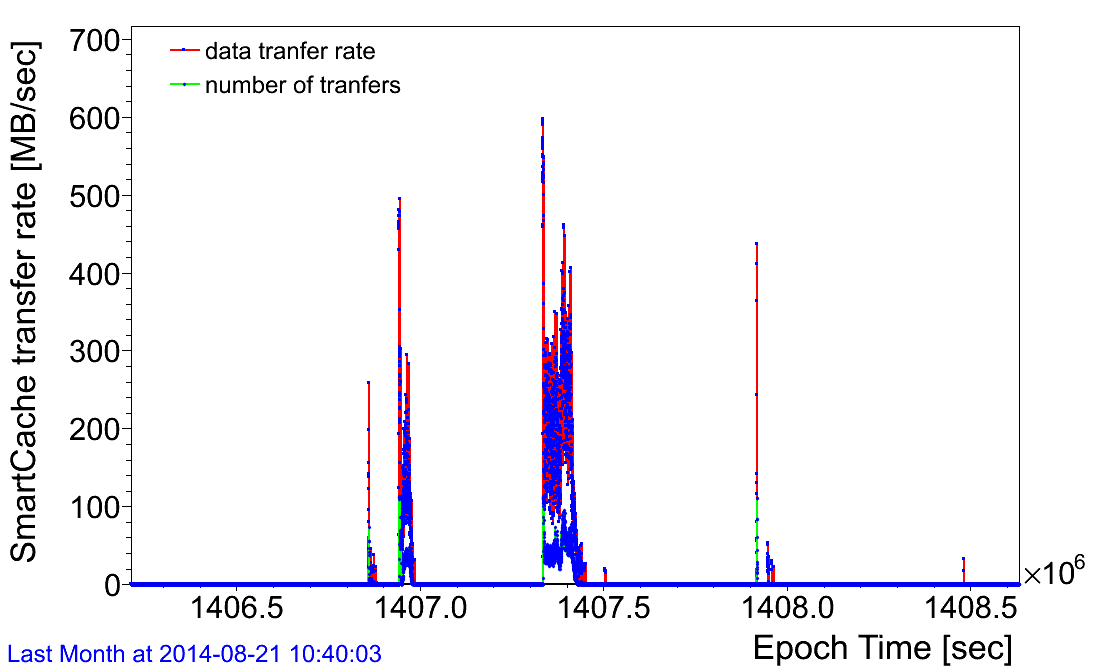
\includegraphics[angle=0,width=0.49\textwidth]{plots/transferRateLastMonth.png}
 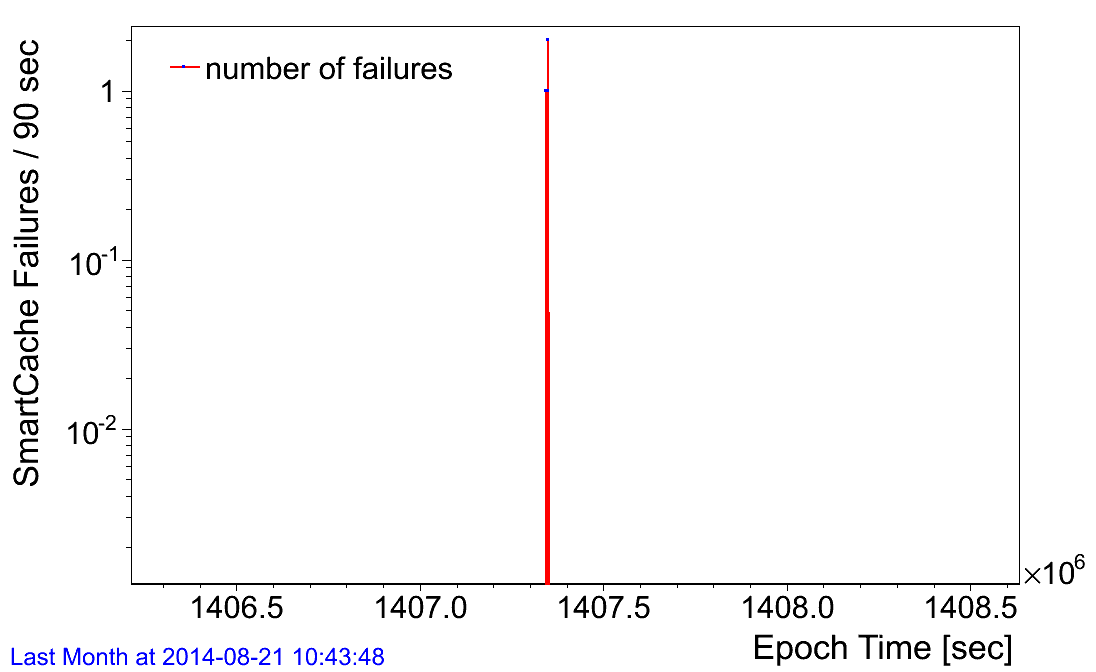
\includegraphics[angle=0,width=0.49\textwidth]{plots/failuresLastMonth.png}
 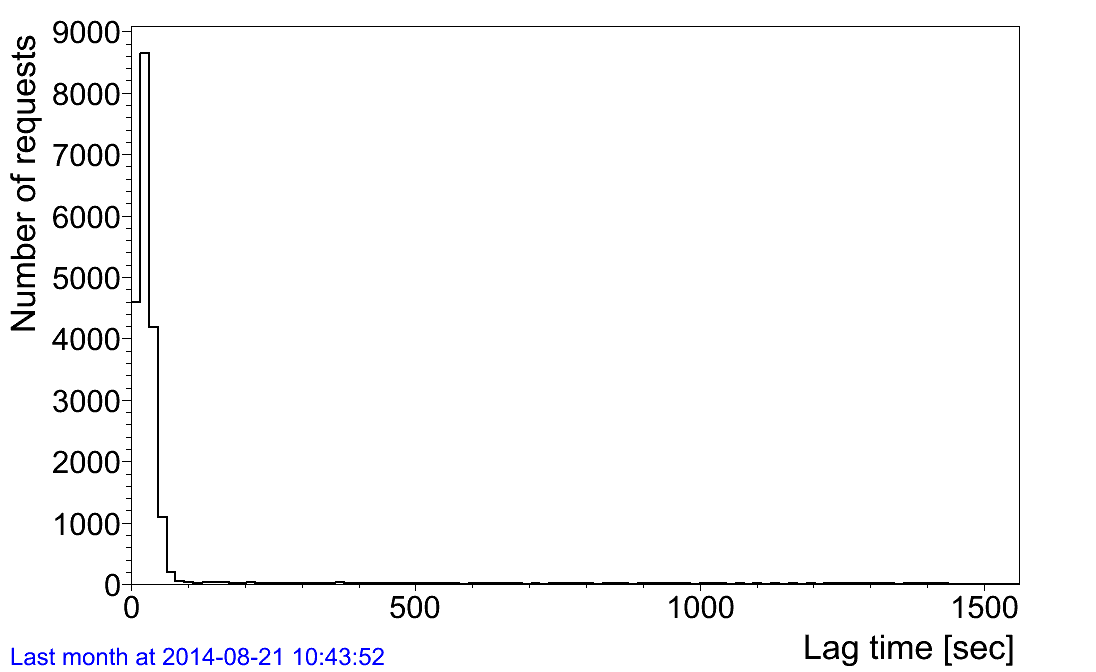
\includegraphics[angle=0,width=0.49\textwidth]{plots/lagTimeLastMonth.png}
 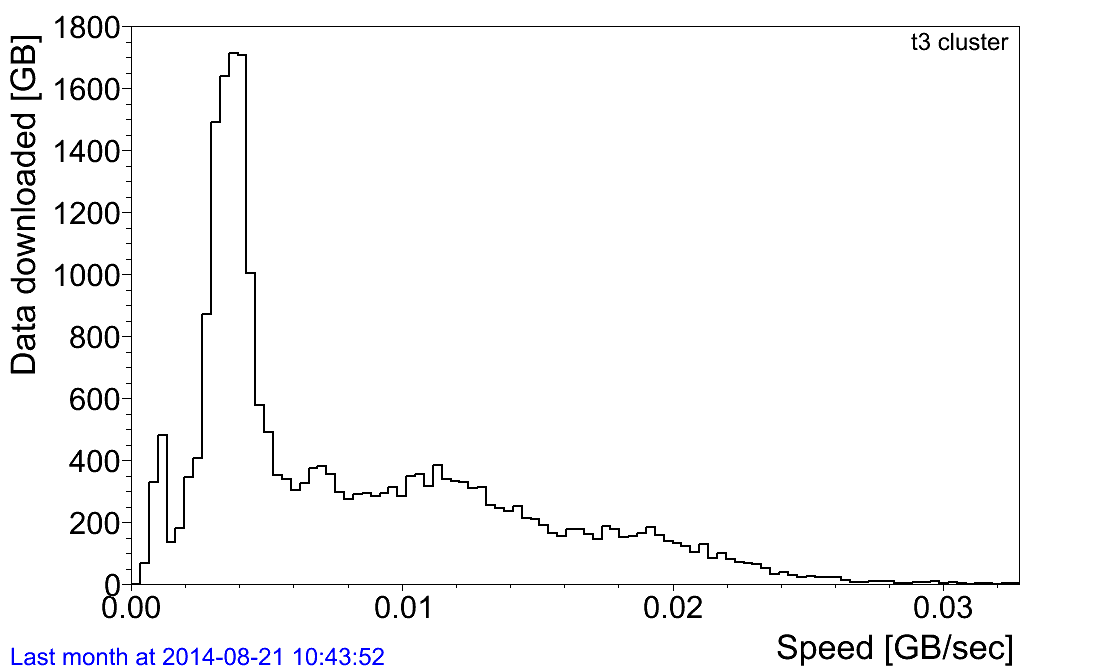
\includegraphics[angle=0,width=0.49\textwidth]{plots/downloadSpeedLastMonth.png}
 \caption{SmartCache monitoring plots for the month of August 2014. In the figures, from top row to bottom row, left to right,
 SmartCache transfer rate, SmartCache transfer failures, Lag time and Speed.}
 \label{fig:SmartCache}
\end{figure}

For of our site, it is interesting to look at Figure~\ref{fig:SmartCache} top-left. First of all it 
shows that we can cache datasets at a total speed of about 5 Gb/s. In addition, we could possibly improve this by
adding more machines to our cacher pool:
at T3\_US\_MIT there are currently 33 machines dedicated to transfers, each carrying an average of three slots, 
thus up to about 100 transfers can happen. Even considering the bandwidth limitation of each machine, we would expect
to be able to saturate our uplink speed, i.e. 8 Gb/s. Nevertheless, the
rate plot shows that the maximum caching speed saturates at 60\% of the total available bandwidth.
Thus, we are limited by some non-network related factors (likely the disk writing speed on TNs).
